\documentclass[../main.tex]{subfiles}

\graphicspath{{../images/}}

\usepackage[noend]{algpseudocode} % for pseudocode
\usepackage[plain]{algorithm} % float environment for algorithms
% preferred pseudocode style
\algrenewcommand{\algorithmicprocedure}{}
\algrenewcommand{\algorithmicthen}{}

% ``do { ... } while (cond)''
\algdef{SE}[DOWHILE]{Do}{doWhile}{\algorithmicdo}[1]{\algorithmicwhile\ #1}%

% ``for (x in y ... z)''
\newcommand{\ForRange}[3]{\For{#1 \textbf{in} #2 \ \ldots \ #3}}

\begin{document}
\pagestyle{fancy}
\chead{Module 7}
\rhead{Junseo Shin}
\lhead{CSE 4059}


\renewcommand{\thefigure}{\arabic{figure}}
\section*{Reduction}

\subsection*{Questions}

\begin{enumerate}
    \item 3 Applications of reduction:
    \begin{enumerate}
        \item Prefix sum: SAT (Summmed Area Table) which can be used for depth of field blurring.
        \item Computing single values such as max/min, average, or standard deviation.
        \item Physics simulations: e.g. N-body simulations where we need to compute the sum of
        forces acting on a particle.
    \end{enumerate}
    
    \item Since the loading into shared memory does one addition per thread, and in the reduction
    step we have $n = \log_2{\texttt{blockDim.x}}$ steps doing one addition times the stride or as a
    finite geometric sum
    \begin{align*}
        \frac{\texttt{blockDim.x}}{2} + \frac{\texttt{blockDim.x}}{4} + \ldots + 1
        &= a \frac{1 - r^{n}}{1 - r} \\
        &= \frac{\texttt{blockDim.x}}{2} \frac{1 - (1/2)^{\log_2{\texttt{blockDim.x}}}}{1 - 1/2} \\
        &= \texttt{blockDim.x} \qt(1 - \frac{1}{\texttt{blockDim.x}}) \\
        &= \texttt{blockDim.x} - 1
    \end{align*}
    so we have $(2 \times \texttt{blockDim.x} - 1) \times \texttt{gridDim.x}$ additions in total.

    \item All the reads are done in the shared memory step which loads 2 elements per thread, so
    we have $2 \times \texttt{blockDim.x} \times \texttt{gridDim.x}$ reads in total or $2 \times N$
    for an input size $N$.

    \item The writes are done once per block when the \texttt{threadIdx.x == 0} so
    we have $\texttt{gridDim.x}$ (number of blocks) writes in total.

    \item Min: If $\texttt{i >= len}$ then we would have 0 real operations. Max: The thread would 
    have 1 addition in the shared step and $\log_2{\texttt{blockDim.x}}$ additions in the reduction
    step. Average: The average number of operations is the result in a block size from 2. divided by
    the number of thread in a block:
    \begin{align*}
        \frac{2 \times \texttt{blockDim.x} - 1}{\texttt{blockDim.x}}
        &= 2 - \frac{1}{\texttt{blockDim.x}}
    \end{align*}
    \newcommand{\floor}[1]{\left\lfloor#1\right\rfloor}
        \item The thread block will synch $\floor{\log_2{\texttt{blockDim.x}}}$ times in the reduction
        step.

    \item The shared memory reduces the the number of global memory accesses to zero in the 
    reduction step!

    \item We could use segmented multiblock sums and/or thread coarsening for faster DRAM access.

    \item We couuld modify the kernel with a grid-stride loop to really large input sizes that are
    bigger than the max dimensions, or use the segmented multiblock sum.

    \item No, we can not use non-commutative operation because the threads will be mixing up the
    order of the operations as it runs in parallel.

    \item Yes, the floating point arithmatic is not associative, so the order of the operations
    will affect the result.

\end{enumerate}

\newpage
\subsection*{OUPUT}
\begin{figure*}[ht]
    \centering
    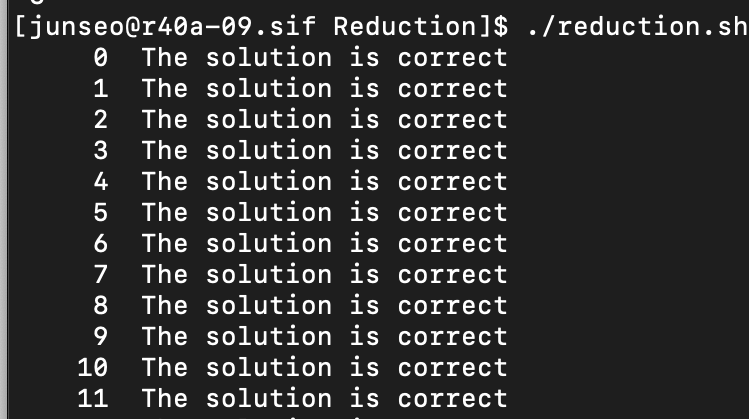
\includegraphics[width=0.8\textwidth]{reduction.png}
    \caption{Successes}
    \label{fig:texthistogram}
\end{figure*}

\end{document} 